Final results of this thesis is presented. As the result acts as
`expected' limits, the ongoing work and potential interpretation are discussed.
\pagebreak
% TODO
% 1) where it intersects -2deltaNLL=3.84
% 2) what is the value of -2deltaNLL at muoffshell=0
\section{Limits on Higgs decay width}
\begin{figure}[htb]
    \centering
    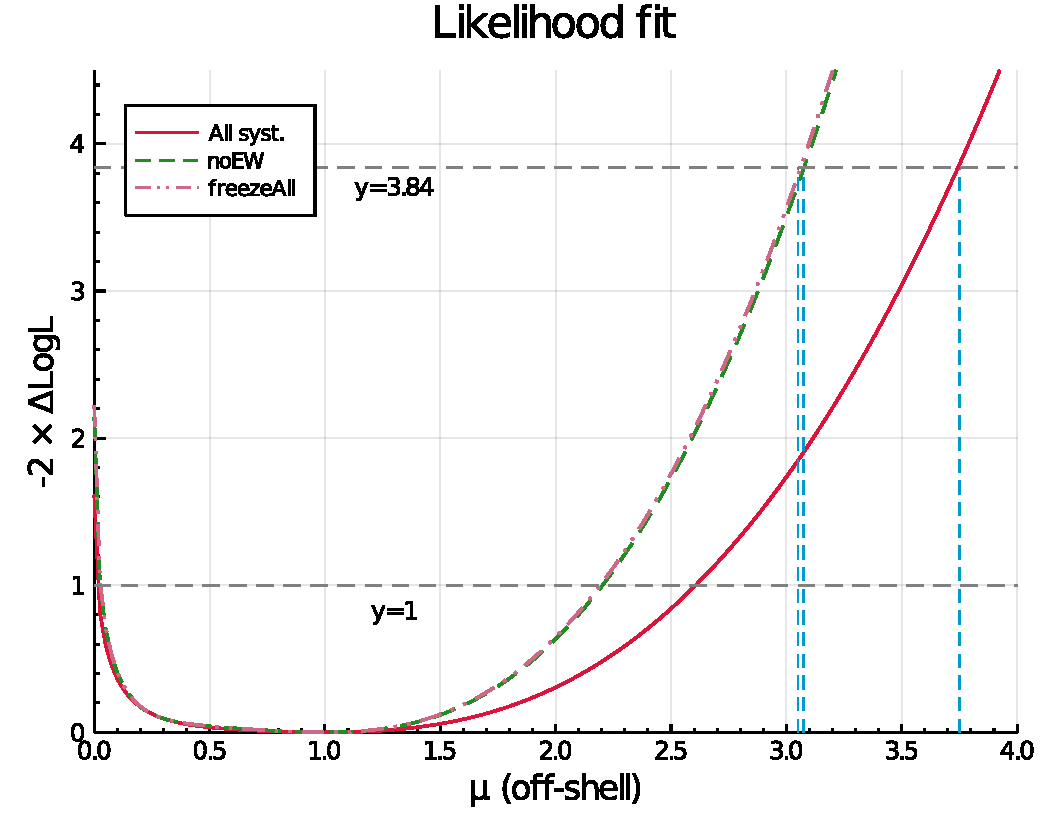
\includegraphics[width=.8\linewidth]{fig/Final_fit_mu_offshell.pdf}
    \caption{Maximum likelihood fit of $\mu^\mathrm{H}_\mathrm{off-shell}$ (off-shell rate ratio).
    For all systematics (red), no Electroweak syst.~(green),
    0 syst.~(orange): y-intersect=\{1.61, 2.14, 2.22\}, 1$\sigma$ lower limits=\{0.025, 0.025, 0.025\},
1$\sigma$ higher limits=\{2.6, 2.2, 2.2\}, 95\% CL limits=\{3.75, 3.08, 3.05\}, respectively.}
    \label{fig:final_fit_mu}
\end{figure}
After running through Combined Limited tool for likelihood fitting, we first extract the significance
of the off-shell rate.~(Fig.~\ref{fig:final_fit_mu})
The y-axis is understood to be $\sigma^2$ in terms of significance, thus
the intersection with the y-axis is the signal sensitivity, or in other words,
rejection of the 0 width hypothesis (no off-shell), which has a significance of 
$\sqrt{1.61} \approx 1.26\sigma$ in this fit with all the systematic uncertainties included.
As the systematics are turned off', the constraint becomes tighter, producing an error band for the expected
final result in the upcoming official anlysis.

\begin{figure}[h]
    \centering
    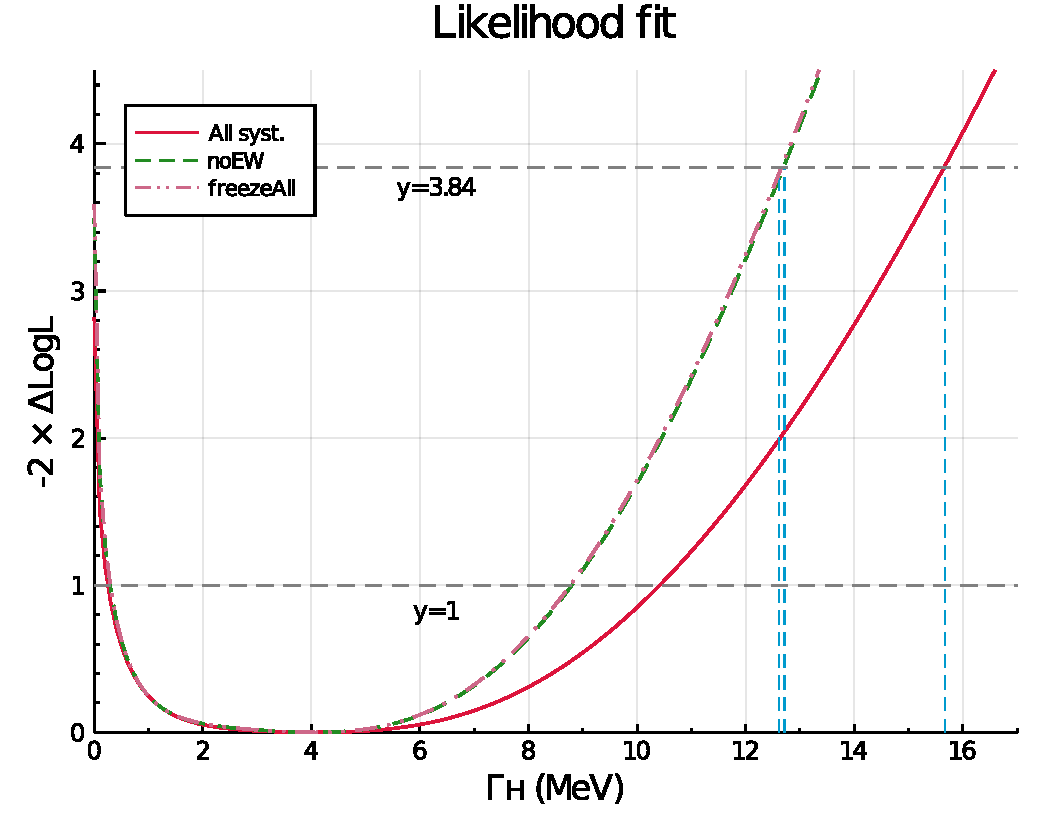
\includegraphics[width=.8\linewidth]{fig/Final_fit_width.pdf}
    \caption{Maximum likelihood fit of Higgs decay width. For all systematics (red), no Electroweak syst.~(green),
    0 syst.~(orange): y-intersect=\{1.61, 2.14, 2.22\}, 1$\sigma$ lower limits=\{0.10, 0.10, 0.10\} MeV,
1$\sigma$ higher limits=\{10.78, 9.16, 9.06\} MeV, 95\% CL limits=\{16.38, 13.33, 13.23\} MeV, respectively.}
\label{fig:final_fit_width}
\end{figure}
Furthuermore, by un-`freezing' the RF=$\mu_\mathrm{F}$ and RV=$\mu_\mathrm{V}$ and adopt the range suggested
\cite{rfrv_higgs_pas}, the constraint on the decay width of Higgs $\Gamma_\mathrm{H}$ is shown in 
Fig.~\ref{fig:final_fit_width}. The minimal (max likelihood) falls on \SI{4.07}{\mega\electronvolt},
consistent with the Standard Model hypothesis being used. 
Again, 1$\sigma$ and 95\% CL are marked respectively. And a final result of 
$\Gamma_\mathrm{H}<\SI{16.38}{\mega\electronvolt}$ shall be quoted.




% without that, what you are showing is actually off-shell signal strength with the assumption that the ratio 
% of the signal strengths for gg and EW productions are as in the SM.
